\documentclass[11pt,a4paper]{article}
\usepackage{fontspec}
\setmainfont{DejaVu Serif}
\usepackage{amsmath,amssymb,graphicx,booktabs,geometry,hyperref}
\geometry{margin=22mm}
\sloppy
\setlength{\emergencystretch}{3em}
\graphicspath{{results/}}
\begin{document}
\title{Експеримент 2: аналітичні SDF та форма}\author{}\date{27 жовтня 2026}\maketitle

\section*{Геометричні еталони}
Знак від'ємний усередині тіла. Для кола та сфери
$d(x)=\|x\|-R$, $R=0.55$. Для квадрата з півстороною $a=0.48$:
\[
 q=|x|-a,\qquad d(x)=\|\max(q,0)\|+\min(\max_i q_i,0).
\]
Два неперетинні диски мають центри $(\pm0.4,0)$ і радіус $0.32$;
точна SDF об'єднання дорівнює мінімуму двох SDF. Ця формула не
оголошується точною для довільних перекритих тіл.
Перешийок --- простий багатокутник із шириною центрального мосту
$0.2$; модуль відстані обчислено мінімумом відстаней до сегментів,
знак --- тестом належності багатокутнику. Це точна евклідова SDF
з точністю арифметики, а не наближене CSG-змішування.
Для тора $R=0.52$, $a=0.20$:
\[
 d(x,y,z)=\sqrt{(\sqrt{x^2+y^2}-R)^2+z^2}-a.
\]
Поворот і зсув реалізовано оберненим жорстким перетворенням запиту.
Квадрат і перешийок мають кути, тому до них не можна глобально
застосовувати припущення про гладку поверхню. SDF також недиференційовна
на відповідних медіальних множинах.

\section*{Обчислення та результати}
$h=0.2$, $r/h=2$, $n=2$, запас $r$, поворот $25^\circ$,
зсув $0.03$ уздовж $x$. Центри та вузли збігаються.
Незалежна сітка оцінки: $151^2$ або $35^3$.
Похибка у смузі означає RMSE за точками $|d-t|<0.2$.
Компоненти визначаються для множини $f\le t$ зі зв'язністю по осях.
\begin{center}\small\resizebox{\linewidth}{!}{\begin{tabular}{llllll}\toprule
Форма & $N$ & RMSE смуги & Помилка знака & Компоненти d & Компоненти f\\\midrule
circle & 225 & 0.01073 & 0.006798 & 1 & 1\\
square & 225 & 0.01397 & 0.009868 & 1 & 1\\
two\_circles & 225 & 0.01427 & 0.01101 & 2 & 2\\
neck & 225 & 0.02562 & 0.03346 & 1 & 1\\
sphere & 3375 & 0.02984 & 0.006577 & 1 & 1\\
torus & 3375 & 0.0307 & 0.01192 & 1 & 1\\
\bottomrule\end{tabular}}\end{center}
Це початкові дискретні вимірювання. Вони характеризують вибрані
параметри, а не весь метод. Кількість компонент залежить від
роздільності сітки. Червона лінія --- рівень моделі, чорна --- еталона.
\begin{center}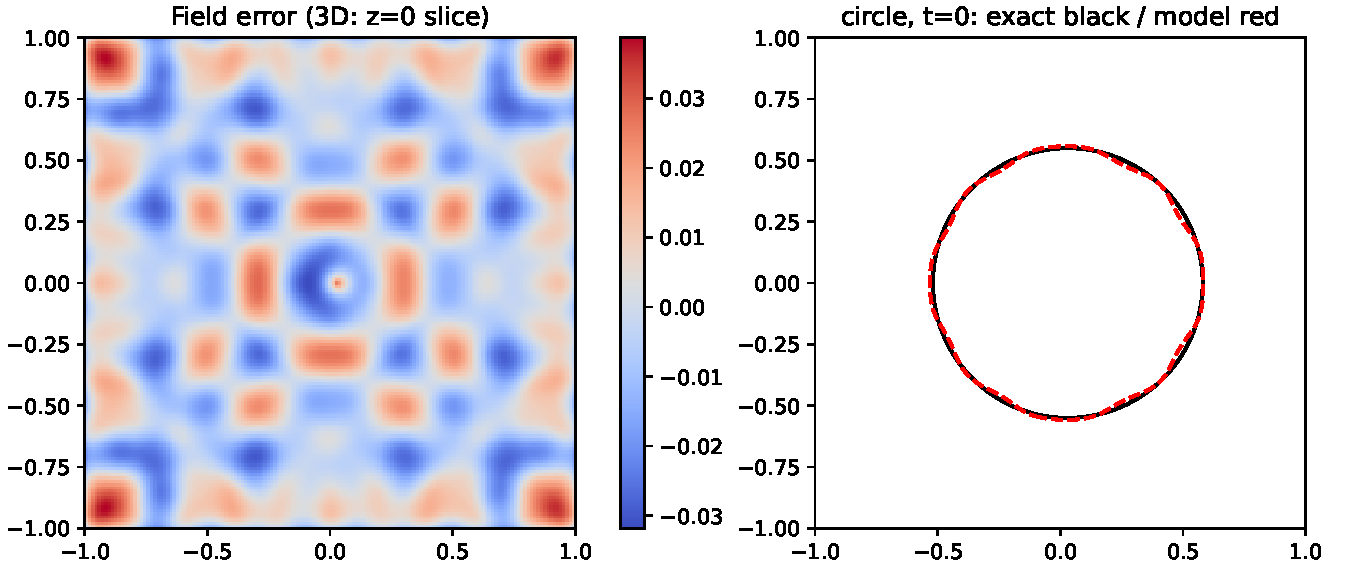
\includegraphics[width=.9\linewidth]{results/experiment2_circle.pdf}\end{center}
\begin{center}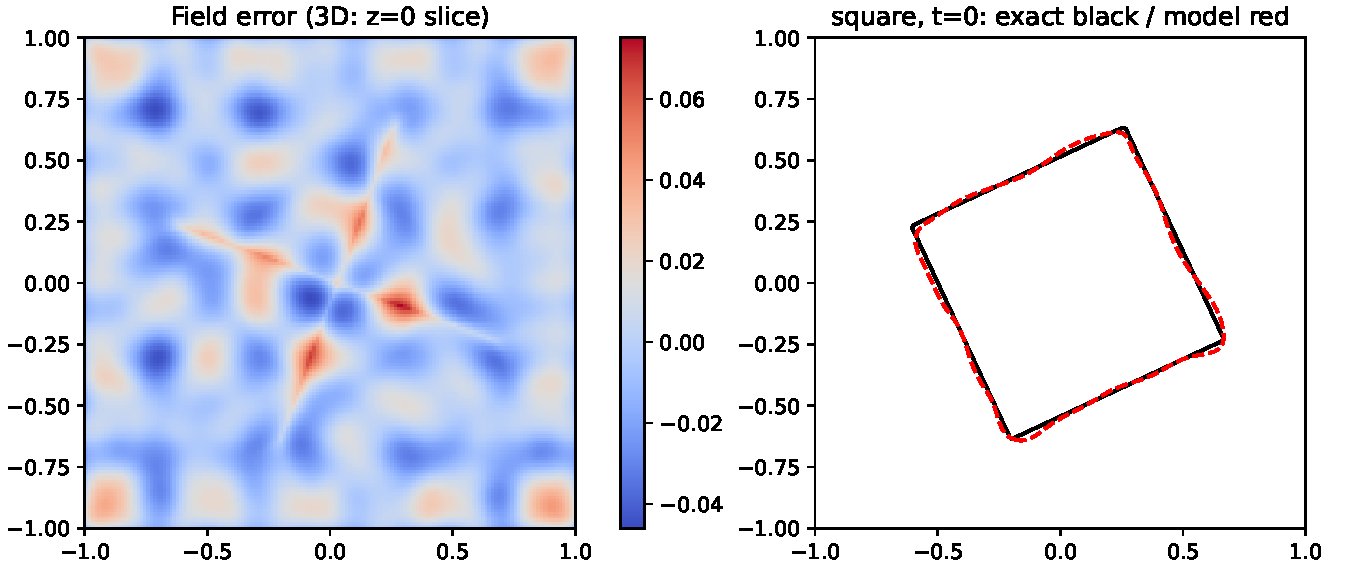
\includegraphics[width=.9\linewidth]{results/experiment2_square.pdf}\end{center}
\begin{center}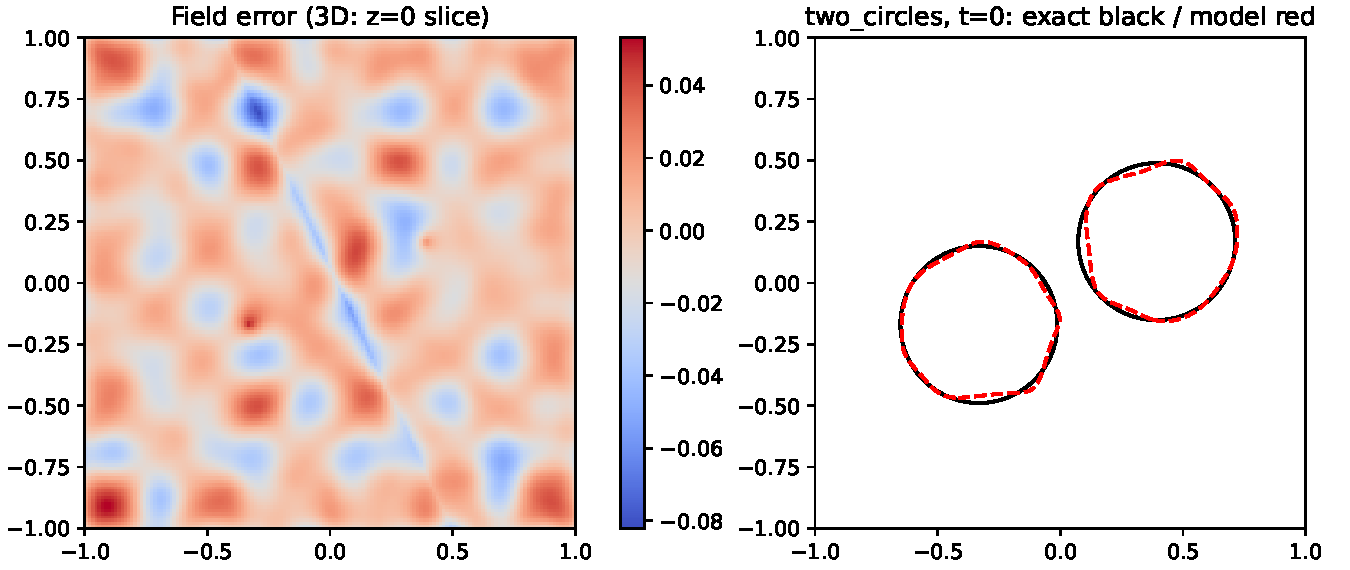
\includegraphics[width=.9\linewidth]{results/experiment2_two_circles.pdf}\end{center}
\begin{center}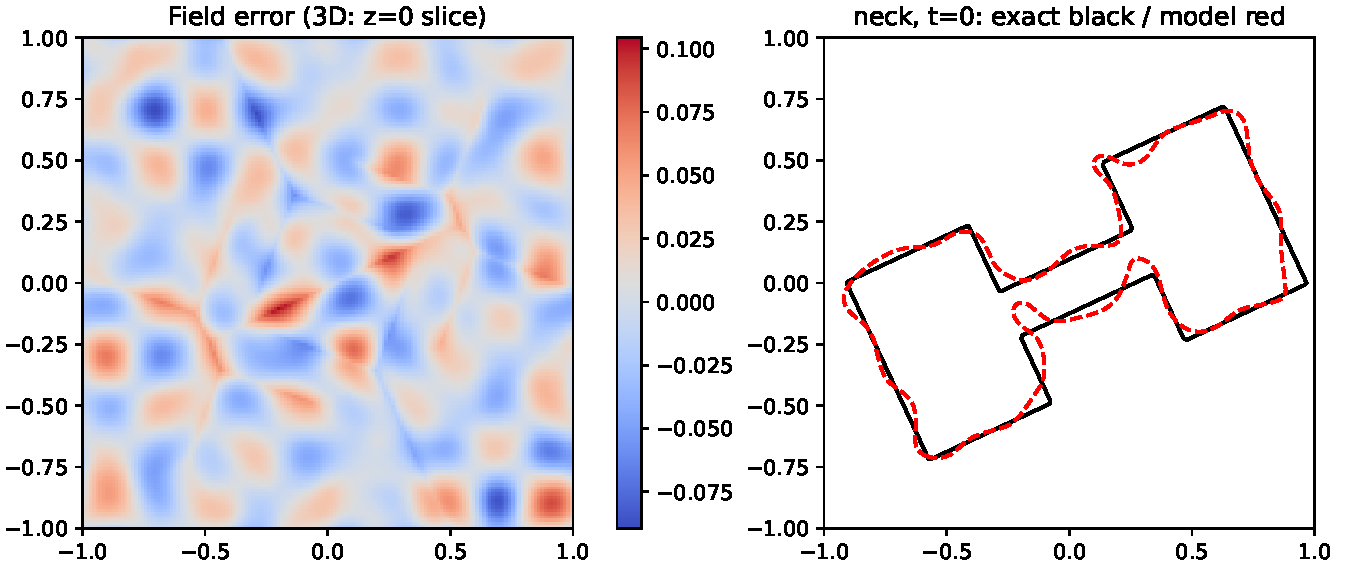
\includegraphics[width=.9\linewidth]{results/experiment2_neck.pdf}\end{center}
\begin{center}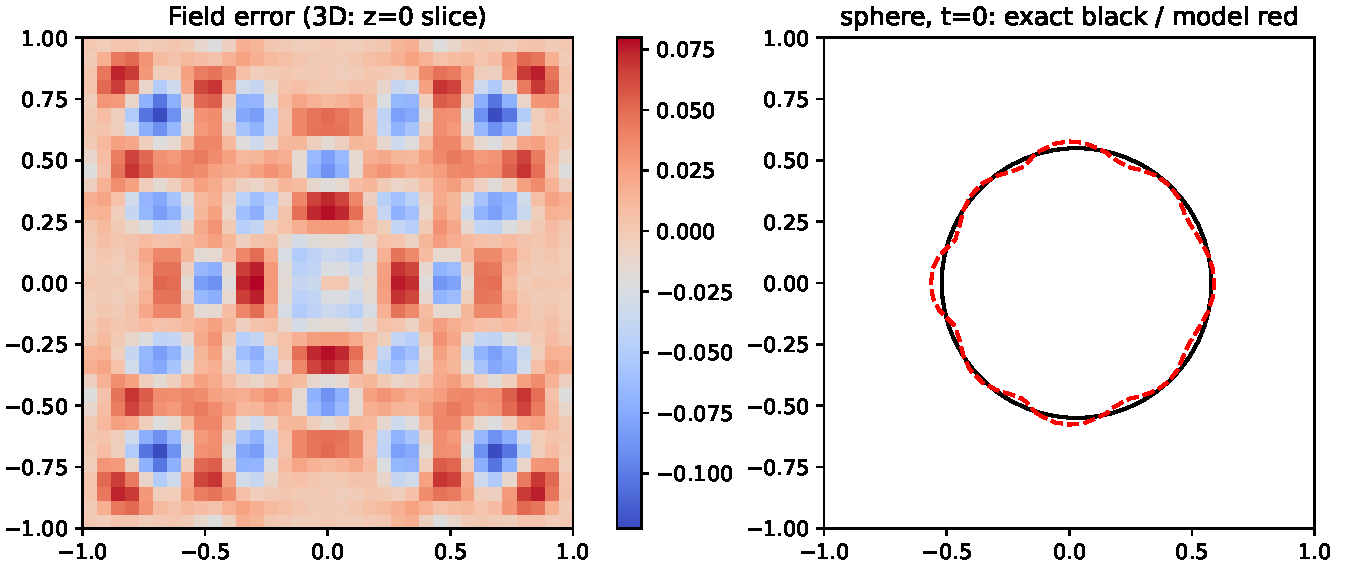
\includegraphics[width=.9\linewidth]{results/experiment2_sphere.pdf}\end{center}
\begin{center}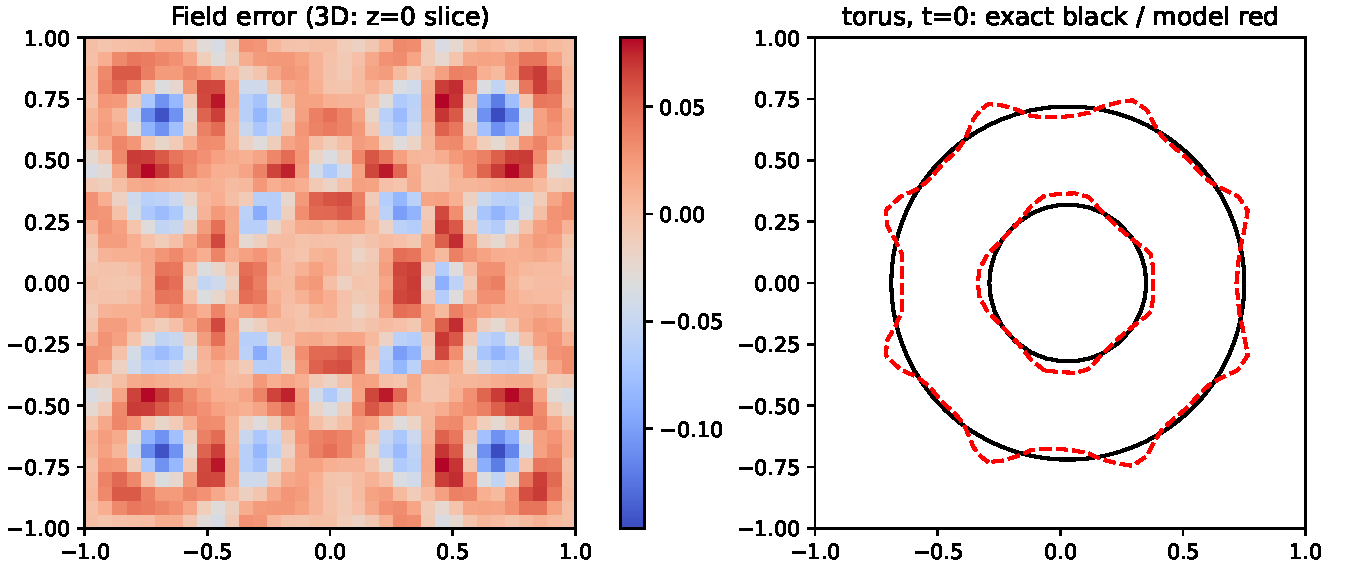
\includegraphics[width=.9\linewidth]{results/experiment2_torus.pdf}\end{center}

Для 3D також побудовано об'ємні ізоповерхні методом marching cubes.
Цей крок додає дискретизаційну похибку; він не змінює самого поля.
\begin{center}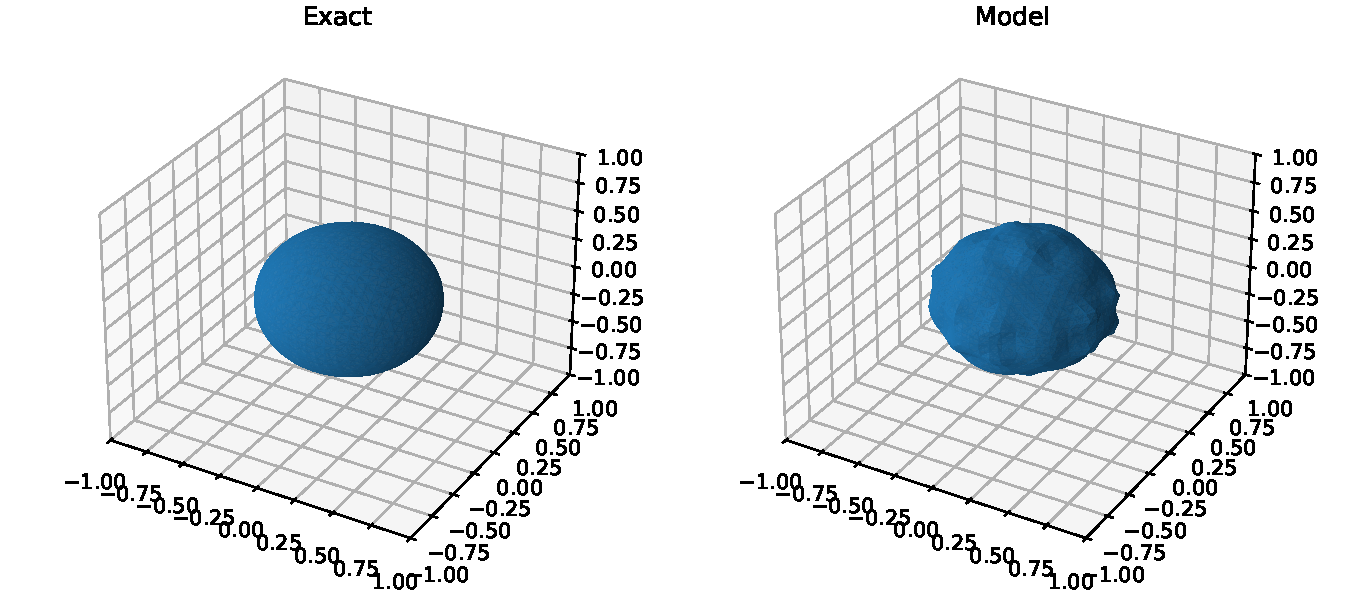
\includegraphics[width=\linewidth]{results/experiment2_sphere_3d.pdf}\end{center}
\begin{center}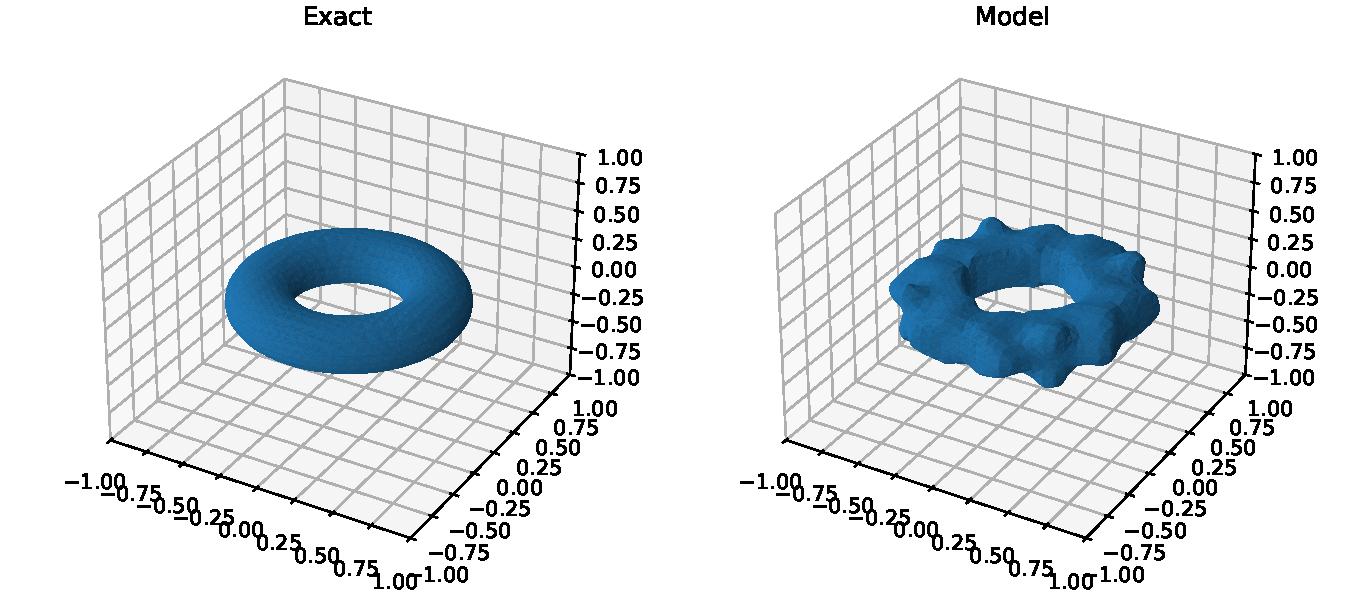
\includegraphics[width=\linewidth]{results/experiment2_torus_3d.pdf}\end{center}

\end{document}
